%! TEX root = ../main.tex
\documentclass[../main.tex]{subfiles}

\begin{document}
\chapter{July 2nd to July 7th, 2025}
First meeting conducted today, introduced to Biruk and the project. I will be mainly focusing on mount calibration.

\section{This week's goals}
List here your goals for this week (to be done by the start of the week).
\begin{enumerate}
    \item Read the three papers
    \begin{enumerate}
        \item     \href{https://imperiallondon-my.sharepoint.com/personal/damato_ic_ac_uk/Documents/Documents/Students%20and%20collaborators/UROP/UROPs%202024-25/Martin%20Leung/References/Kaygorodov_submitted_250325.pdf?CT=1751483727407&OR=ItemsView}{ConferencePaper}
        \item     \href{https://imperiallondon-my.sharepoint.com/personal/damato_ic_ac_uk/Documents/Documents/Students%20and%20collaborators/UROP/UROPs%202024-25/Martin%20Leung/References/FYP%20report%20-%20Kaygorodov%20Egor.pdf?CT=1751483722224&OR=ItemsView}{FYP report - Kaygorodov Egor}
        \item     \href{https://imperiallondon-my.sharepoint.com/personal/damato_ic_ac_uk/Documents/Documents/Students%20and%20collaborators/UROP/UROPs%202024-25/Martin%20Leung/References/FYP%20report%20-%20Hjelmstad%20Rattigan%20Mathias.pdf?CT=1751483719135&OR=ItemsView}{FYP report - Hjelmstad Rattigan Mathias}
    \end{enumerate}

    \item Read \href{https://imperiallondon-my.sharepoint.com/personal/damato_ic_ac_uk/Documents/Documents/Project%20management/CICLOPS/Documentation/AZ1000HPS-Mount-Manual.pdf?CT=1751488182511&OR=ItemsView}{10Micron mount manual}
    \item and the other \href{https://imperiallondon-my.sharepoint.com/:w:/r/personal/damato_ic_ac_uk/_layouts/15/Doc.aspx?sourcedoc=%7B8D6E4E67-449D-424F-AB04-5AF75790CAC8%7D&file=Martin%20Leung%20-%20Meeting%20notes.docx&action=default&mobileredirect=true}{minutes} stuff
    \item \href{https://imperiallondon-my.sharepoint.com/personal/damato_ic_ac_uk/_layouts/15/onedrive.aspx?id=%2Fpersonal%2Fdamato%5Fic%5Fac%5Fuk%2FDocuments%2FDocuments%2FProject%20management%2FCICLOPS%2FDocumentation&CT=1751483599340&OR=OWA%2DNT%2DMail&CID=a9e9192b%2D8bd2%2D9e4f%2Db0e7%2D1bfa1679f5b3&e=5%3A37a1453353a044b38a1eb021c49fdaa6&sharingv2=true&fromShare=true&at=9&FolderCTID=0x012000A0D128FDFD328A43BB09E3D870B16404&view=0}{CICLOPS documentation with mount notes by Dr Amato}
\end{enumerate}
\section{Quick notes and jots}
\begin{enumerate}
    \item Platesolve2 requires: PlateSolve2, APM Star Catalog. \href{https://astroguide.starlust.de/html/PlateSolve2.html}{Guide}.
    \\ Notes
    \begin{itemize}
        \item APM is installed in \verb|C:\Program Files (x86)\Starry Ridge\APM|
        \item Test images can be generated with \href{https://gea.esac.esa.int/archive/}{ESA Gaia Archive} as suggested by \href{https://www.cloudynights.com/topic/886389-here-is-a-useful-tool-to-obtain-known-good-test-images-for-plate-solving/}{this post}. Go to "Single object" at top left navigation bar, move to a position in the sky and FOV then simply use the camera function.
    \end{itemize}
    \item \href{https://10micron.eu/en/downloads/modelcreator}{ModelMaker} (bottom right of the page) is made by Per Frejvall, same guy who made this \href{https://www.youtube.com/watch?v=WfkQnZTFXzo}{youtube video}. However, it is old and he died "some years ago". It requires GSC1.1, which is downloded like this:
    \begin{itemize}
        \item Download \href{https://eternallybored.org/misc/wget/}{wget} and put it in \verb|C:\wget|
        \item Use this command:\\ \verb|wget -r -np -nH --cut-dirs=4 -R "index.html*" -P C:/GSC11 https://cdsarc.u-strasbg.fr/ftp/cats/bincats/GSC_1.1/|
        \item CHATGPT explains the options: \\
        -r	Recursively download all files\\
        -np	No parent — stay within the specified directory\\
        -nH	Don't create a folder for the hostname (cdsarc.u-strasbg.fr)\\
        --cut-dirs=4	Strip 4 directory levels to flatten the output into C:/GSC11\\
        -R "index.html*"	Skip auto-generated index files\\
        -P C:/GSC11	Save everything into C:/GSC11\\
    \end{itemize}
        \item \href{https://10micron.eu/en/downloads/modelcreator}{ModelCreator} is what we will use from now on I believe
        \item can book \href{https://imperial.siso.co/ui/search-basket.php}{SISO} room, flight arena, apparently lending charge of 56 quid?
        \item \href{https://ascom-standards.org/Downloads/Index.htm}{ASCOM Platform 7.0} Not really sure how this works, will have to ask amato.
        \item 10Micron forums have been registered, awaiting admin approval. \href{https://forum.10micron.eu/}{10Micron Forum}
        \item SharpCap for interfacing with the camera and mount, and for polar alignment. \href{https://www.sharpcap.co.uk/sharpcap/downloads}{SharpCap Downloads}
        \item Risk assessments goes here I think \href{https://imperiallondon.sharepoint.com/sites/foe/aero/safety/General%20Risk%20Assessments/Forms/MyItems.aspx}{Imperial College Aero Risk Assessments}
        \item Night at London right now is around 10pm for stars to be visible, good luck... Visible stars are likely Vega, Arcturus, Deneb.
        \item Looking from \href{https://imperiallondon-my.sharepoint.com/:w:/r/personal/damato_ic_ac_uk/Documents/Documents/Project%20management/CICLOPS/Documentation/Manual_v1.docx?d=wb7504c9d211b4b098ad126b4b6c34f2e&csf=1&web=1&e=2N7g7I}{Manual v1} from the documentation folder, focusr motor might need to be calibrated with \href{https://www.celestron.com/pages/celestron-pwi-telescope-control-software}{Celestron PWI Telescope Control Software}
\end{enumerate}
\section{Downloaded software (Only the ones I think I need)}
\begin{itemize}
    \item \href{https://astroguide.starlust.de/html/PlateSolve2.html}{PlateSolve2}
    \item \href{https://astroguide.starlust.de/html/PlateSolve2.html}{APM Star Catalog}
    \item \href{https://10micron.eu/en/downloads/modelcreator}{ModelCreator}
    \item \href{https://ascom-standards.org/Downloads/Index.htm}{ASCOM Platform 7.0}
    \item \href{https://www.sharpcap.co.uk/sharpcap/downloads}{SharpCap}
    \item \href{https://www.celestron.com/pages/celestron-pwi-telescope-control-software}{Celestron PWI Telescope Control Software}
\end{itemize}
\section{Other downloaded software}
\begin{itemize}
    \item \href{https://10micron.eu/en/downloads/modelcreator}{ModelMaker}
\end{itemize}
\section{Preliminary Knowledge}
Just to remind myself, right ascention and declination is measured off the vernal equinox along the equatorial plane in inertial frame. Whereas azimuth is measured as angles from the north point of the horizon clockwise, and elevation is measured from the horizon up to the object in the sky in the position of the observer.

\begin{figure}[h]
    \centering
        \begin{minipage}{0.45\textwidth}
        \centering
        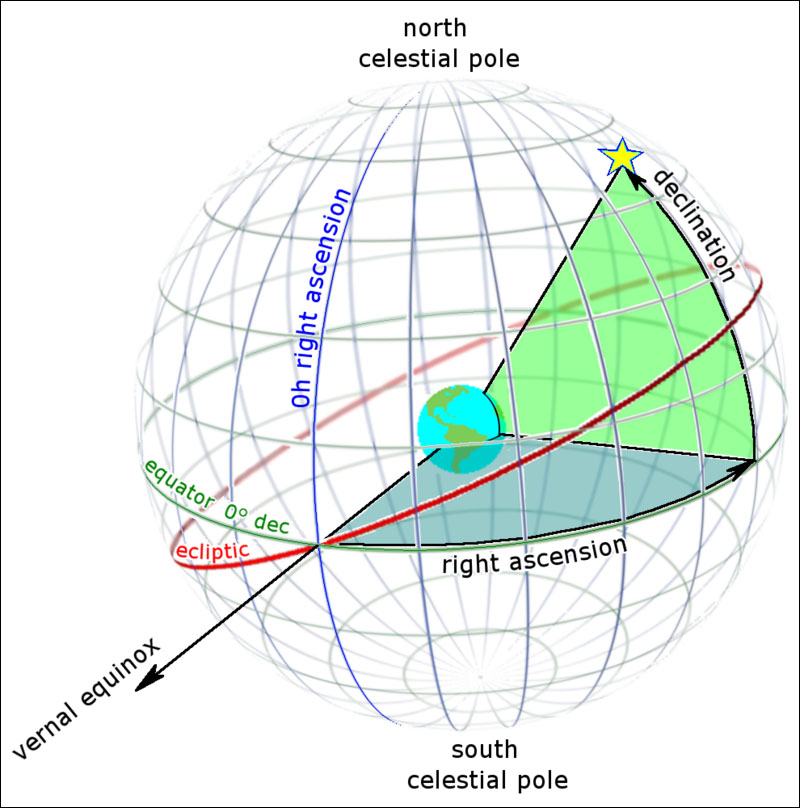
\includegraphics[width=\textwidth]{radec.jpg}
        \caption{Right Ascension and Declination.}
        \label{fig:radec}
    \end{minipage}
    \hfill
    \begin{minipage}{0.45\textwidth}
        \centering
        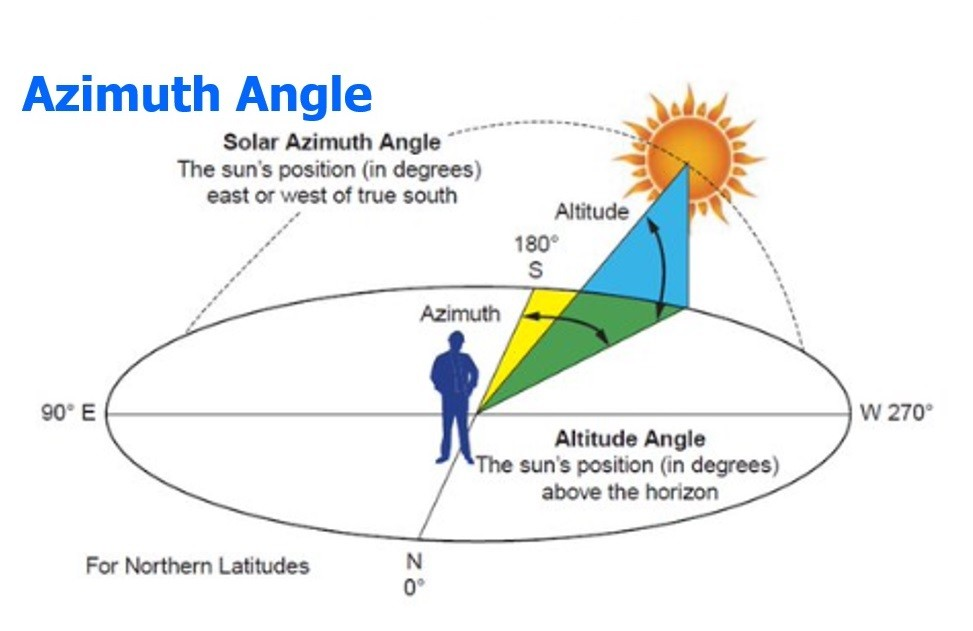
\includegraphics[width=\textwidth]{azialt.jpeg}
        \caption{Azimuth and Elevation.}
        \label{fig:azialt}
    \end{minipage}
    % \caption{Main caption for both figures}
    % \label{fig:orbiter_figures}
\end{figure}
\section{Literature Review}
Just quick notetaking for the papers I read this week.
\subsection{Conference Paper}
\begin{itemize}
    \item SSA using 10Micron AZ1000HPS mount with 1 arcsecond accuracy, but without proper calibration it can be $~3\deg$ off.
    \item Workflow: User > OST > Mount Control > (Mount Control + GPS Tracker + Camera + Astrograph) > Image Processesor > output
    \item Image Processor: Camera > SharpCAP > Background Removal >
    \begin{itemize}
        \item Streak identification
        \item Platesolve2
    \end{itemize}
    > Data Processesor > Object visual magnitude + object angular parameters
    \item OST uses ESA's DICOS database with 15000 objects are propagated with SGP4 to find passes using many masks and filters.
    \item Mount calibration uses ~10 star alignment. (Non orthogonal axes cannot be compensated for so must be shimmed if errors are too large)
    \item Accuracy is expected to be superior to that of "Propagated TLEs"
    \item Future: Use pyPOGS with mount control, image capture and reduction. (Repo is 3-6 years old...)
\end{itemize}
\subsection{FYP Report - Hjelmstad Rattigan Mathias}
\begin{itemize}
    \item Balance reading of less than 0.4\% is optimal, done thorugh Menu>Alignment>Balance on keypad.
    \item TLEs are uploaded to 10Micron
    \item Most the report is on OST and using it to estimate theoretical errors in tracking by perturbuing orbital elements.
    \item A lot of SOP is here!
\end{itemize}
\subsection{FYP Report - Kaygorodov Egor}
\begin{itemize}
    \item I couldn't really use much of this information, 99\% of it is focused on image processing.
\end{itemize}
\subsection{Mount Manual}
\subsubsection{Saftey}
\begin{itemize}
    \item Never look at the sun, never let it ever look in the sun or near it. Do not leave unattended for this reason.
    \item Make sure mount is stable and locked when mounting astrograph or counterweights.
    \item Never move "declination axis" from "safety position with counterweights mounted but without telescope mounted on other side" ?? What is declination axis?
    \item Balancing error can lead to damages
    \item DO not tighten clutches too much, tracking performance degration
    \item All connections except LAN must be made before connecting power. As such dont disconnect when power on.
    \item Prevent tangling cables from rotating parts. Move manually to check
    \item Clock battery must be 3V Lithium CR2032 non rechargable.
    \item Do not slew greater than 10deg/s, if needed dont stay near it
    \item Firmware upgrades might not preserve position memory
    \item Each second of clock error leads to 15 arcseconds of error in position. Adjusted manually, with PC or GPS module. Clock can be adjusted without aligning again.
    \item Not advised to change local data settings while object tracking.
    \item Custom park positions do not have software limits, make sure no collisions can happen.
\end{itemize}
\subsection{Youtube video instruction}
Talks a lot about the history of the mount, pros and cons of different models. The thing I cared about was the operation of model maker, which apparently is just clicking a bunch of points and letting it do its thing?
\end{document}